\begin{figure}[htbp]
\centering
\caption{Predictors of Post-Treatment Bilateral Connectivity}
\label{fig:bilateral_coefplot}

\begin{threeparttable}

\begin{subfigure}{\textwidth}
    \centering
    \caption{Panel A: Univariate Regressions}
    \label{fig:bilateral_coefplot_univariate}
    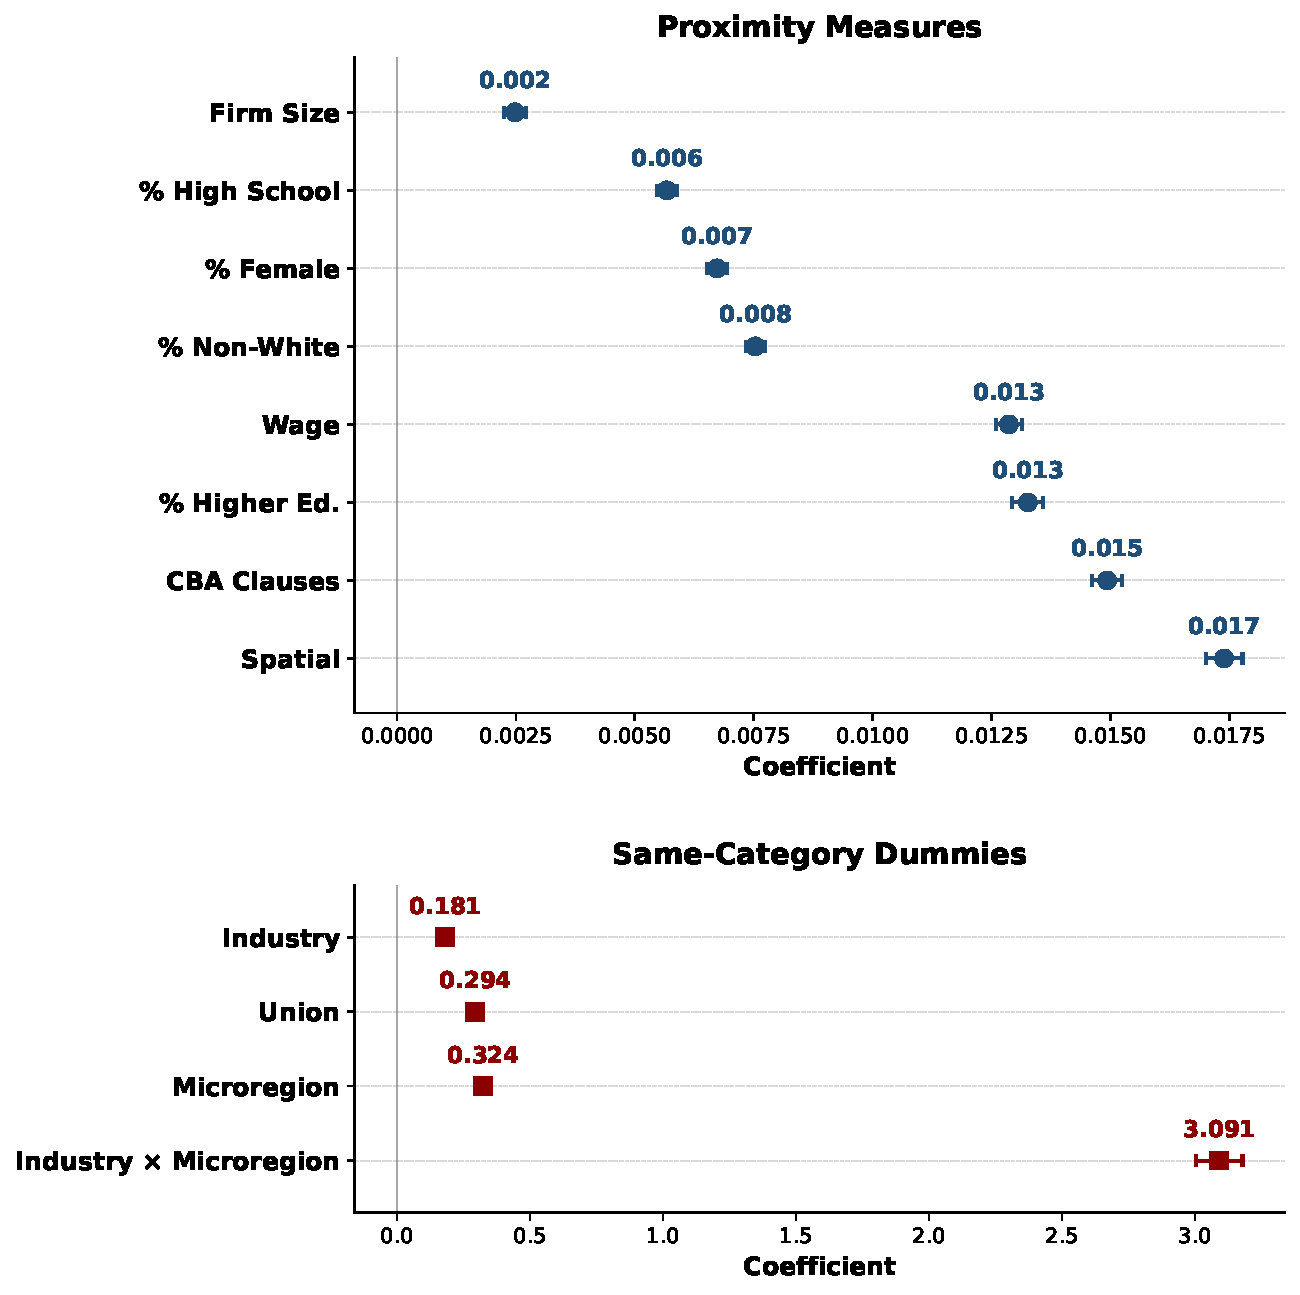
\includegraphics[width=0.85\textwidth]{coefplot_bilateral_univariate.pdf}
\end{subfigure}

\vspace{1em}

\begin{subfigure}{\textwidth}
    \centering
    \caption{Panel B: Multivariate Regression}
    \label{fig:bilateral_coefplot_multivariate}
    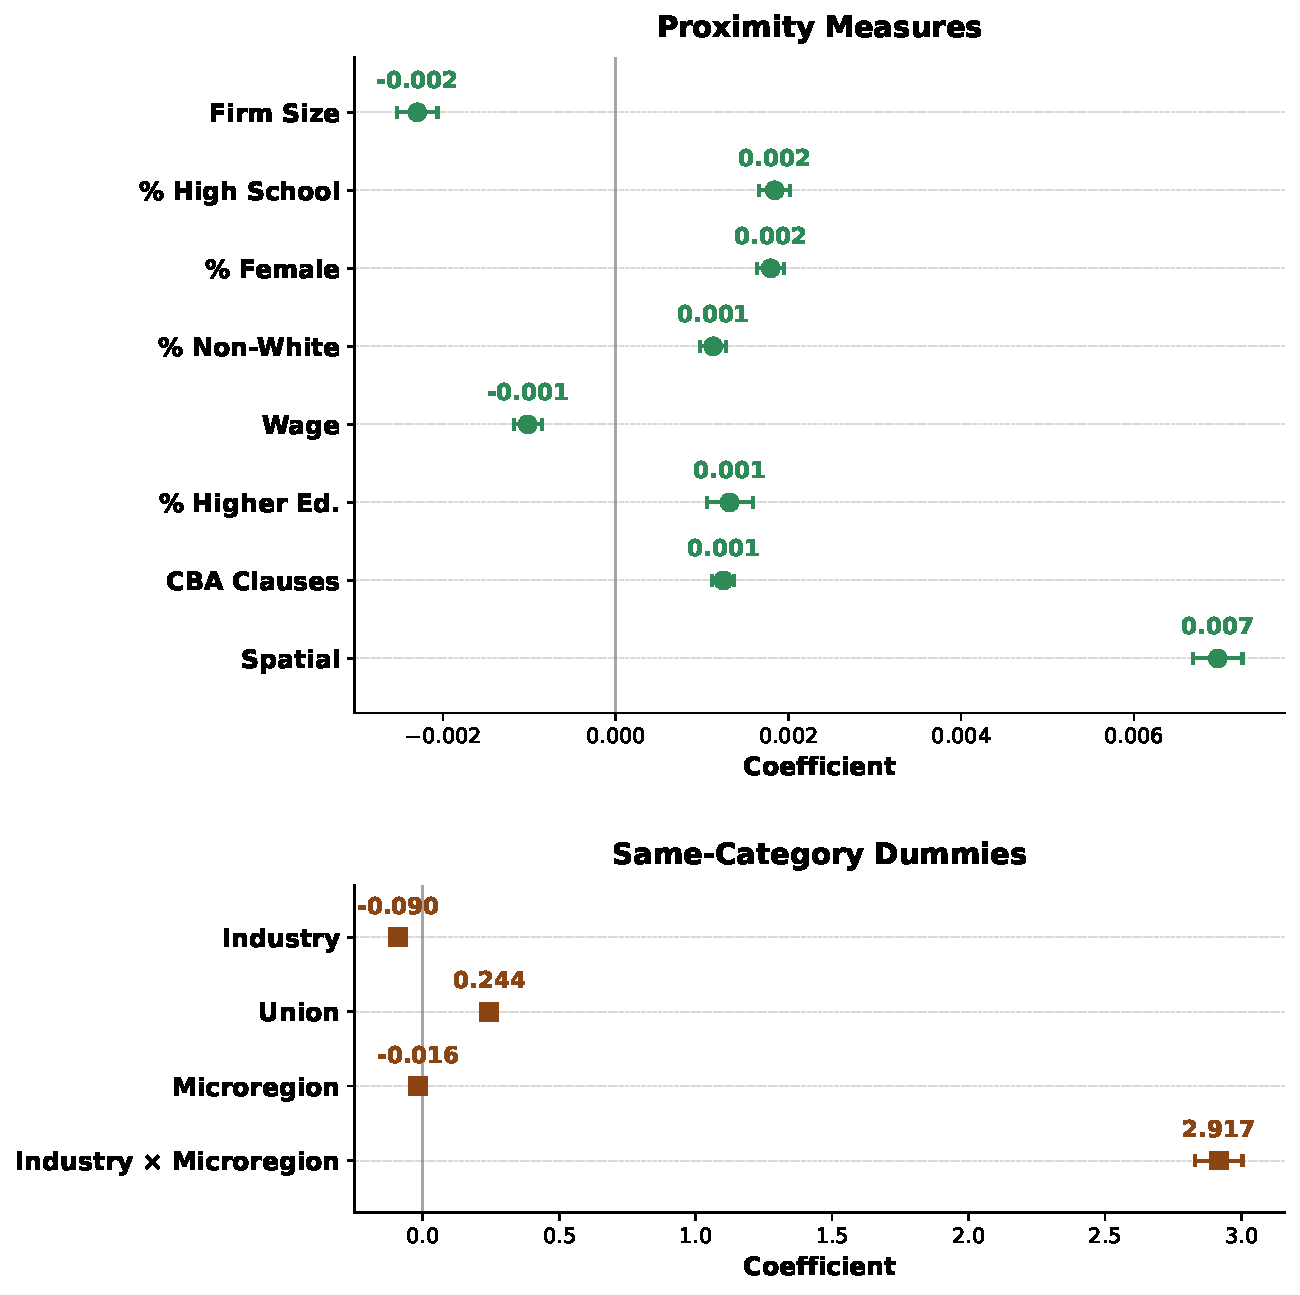
\includegraphics[width=0.85\textwidth]{coefplot_bilateral_multivariate.pdf}
\end{subfigure}

\begin{tablenotes}
\footnotesize
\item \textit{Notes:} Panel A shows coefficients from separate univariate regressions of post-treatment bilateral connectivity (2012--2016) on each indicated predictor. Panel B shows coefficients from a single multivariate regression including all predictors simultaneously. All regressions control for establishment $i$ fixed effects. Bilateral connectivity is measured as the person-weighted average flow of workers between establishment pairs. Proximity measures are defined as the negative absolute difference between establishment characteristics (standardized), so higher values indicate greater similarity. Spatial proximity is measured as the negative log of distance between municipality centroids. CBA clauses proximity is based on the number of clauses in collective bargaining agreements. Same-category dummies equal one if both establishments share the indicated category. Horizontal lines represent 95\% confidence intervals based on robust standard errors. All regressions include the universe of establishment pairs, including those with zero worker flows.
\end{tablenotes}

\end{threeparttable}
\end{figure}
